\begin{bibunit}
\thispagestyle{plain}

% Add missing command definitions from original paper
\newcommand{\commentcolour}[3]{\textcolor{#3}{[\textbf{#1:} #2]}}
\newcommand{\commentVV}[1]{\commentcolour{VV}{#1}{orange}}
\newcommand{\VV}[1]{\textcolor{orange}{#1}}
\newcommand{\soutVV}[1]{\VV{\sout{#1}}}
\newcommand{\corrVV}[2]{\sout{#1} \VV{#2}}
\newcommand{\N}{{\mathbb N}}
\newcommand{\NN}{\mathcal N}
\newcommand{\etal}{\it et al. \normalfont}

\section*{Abstract}

This paper proposes a novel AI agent for reasoning, planning, and testing industrial automation applications. The AI agent accepts operator instructions in natural language and performs semantic reasoning over functional requirements to generate an optimized cost-effective action plan. This plan comprises a sequence of executable actions that can be deployed in industrial control systems (ICS) to enable efficient and sustainable machine operation. Then the AI agent automates the testing of control systems by comparing the agent's planned and executed actions against expected outputs, ensuring requirement conformance and enhancing system reliability. Experimental results demonstrate the effectiveness of the AI agent in generating sustainable operational plans and validating control system behavior for laboratory scale case studies, underscoring its potential in the future of intelligent industrial automation.
    
    
    \section{Introduction}
    \label{Introduction}
    
    Industrial automation systems are the backbone of modern manufacturing and production environments. These systems are essential for improving productivity, consistency, and safety across various industrial sectors. As automation becomes increasingly sophisticated, the need for intelligent decision-making and adaptive control continues to grow \cite{khan2020management}. The integration of artificial intelligence (AI) into industrial automation is a promising direction to meet the evolving demands of efficiency, flexibility, and reliability \cite{mathew2023artificial}.
    
    A rapidly gaining popularity architecture for developing distributed industrial control systems is the IEC 61499 standard, which defines a component-based model using Function Blocks (FBs) \cite{iec61499part12012}. IEC 61499 facilitates modularity, portability, and reusability of control logic, making it suitable for building complex, event-driven automation applications. However, despite its advantages, developing optimal execution plans and verifying the control logic across multiple scenarios remains a time-consuming and error-prone process, especially when scaling up to industrial levels.
    
    The OPC Unified Architecture (OPC UA) has emerged as the standard protocol for secure and reliable communication in industrial systems \cite{OPC_UA_2023}. OPC UA enables seamless data exchange between heterogeneous devices and systems, promoting interoperability across the automation pyramid. By integrating OPC UA with IEC 61499 applications, developers can create connected systems capable of real-time monitoring and control \cite{majumder2023proposal}. Yet, realizing an intelligent and sustainable industrial control system using these technologies still faces significant challenges.
    
    One of the primary challenges in current ICS is the lack of automated tools to generate energy- and cost-efficient operational plans \cite{benedetti2017energy}. Designing control logic that balances operational performance with resource sustainability requires extensive domain expertise and manual tuning. Furthermore, testing and validating ICS against a wide range of requirements---such as safety constraints, expected outputs, and timing behavior---remain labor-intensive \cite{antao2018requirements}. This is due to the informal representation of system requirements, which are typically written in Natural Languages and not machine interpretable. Bridging the gap between automatically translating informal requirements to formal testing sequences will contribute towards reducing the manual intervention required in system testing. Existing solutions often fall short in dynamically adapting to new conditions or verifying compliance with evolving specifications.
    
    This paper addresses these limitations by proposing a knowledge-driven AI agent capable of interpreting natural language instructions, reasoning over system requirements, and generating optimized action plans. In addition, the agent can automatically analyze the industrial control system based on a given set of requirements and expected behaviors, significantly reducing the time and effort required for validation. By leveraging semantic reasoning, the agent transforms operator instructions into executable skill sequences, integrates with IEC 61499 applications via OPC UA, and automates requirement-based testing. Through this approach, the proposed system aims to enhance the \textit{efficiency, sustainability, and reliability} of industrial automation systems, representing a step toward intelligent control in Industry 4.0 environments.
    
    
    
    \section{ Related work}
    \label{sec:background}
    
    Manufacturing-oriented ICS form the backbone of modern factories, tasked with operating machines and processes under strict performance and cost constraints. Recent trends such as mass customization demand that production lines become highly flexible and adaptable, departing from the traditional fixed, high-volume configurations \cite{9576342}. At the same time, efficiency pressures are growing – factories must minimize energy consumption and operational costs while maintaining throughput. The industrial sector is indeed entering “a transformative era of intelligent automation driven by Artificial Intelligence (AI) capabilities,” emphasizing smarter and more autonomous operations\cite{10677409}. 
    
    Engineering effort, required to develop and test functionality of automation systems significantly affects their flexibility and costs. Model-driven software engineering has been widely investigated as the means to increase the efficiency of software engineering thus improving their characteristics. IEC 61499 has been attractive for developers as providing a balanced approach for model-driven development, combining component design, state machines, and sequence diagrams.
    
    On another side, there have been many attempts to improve engineering efficiency by increasing the level of programming, i.e. providing the developer higher level artefacts to operate with. Usually these are implemented as libraries of functions or function blocks. A noteworthy approach was developed to standardise such higher-level design artefacts known as skills. Started from definition of skills as higher-level manufacturing operations in \cite{pfrommer2013pprs}, it was augmented with direct communication with the skills via OPC UA giving a way to engineering. In this paradigm, machine functions are encapsulated as modular “skills” (services) with well-defined interfaces, often following the service-oriented architecture (SOA) principle \cite{9576342}. Research shows that skill-based engineering greatly aids reusability and plug-and-produce integration of new components. Dorofeev \etal demonstrated a generic skill interface that hides low-level device details and “provides a common semantic model for the execution” of manufacturing tasks \cite{10.1145/3377812.3381394}. This semantic modeling of skills enables higher-level planners to reason about operations in human terms (e.g. “assemble part A to B”), rather than device-specific commands. The current skill frameworks still lack deep semantic reasoning – generating an optimized plan from a high-level goal is not trivial. \iffalse Ongoing studies on ontology-based planning for smart manufacturing underscore this point; researchers are developing ontologies to impart common meaning to processes and resources, as a basis for intelligent planning and control \cite{9087396}.... \fi  The persistence of this challenge suggests that, while skill-based architectures provide a foundation for modular and semantic control, we need more powerful reasoning agents to interpret complex goals and constraints and then orchestrate skills optimally in response to new production demands. 
    
    Energy-efficient operation and planning in industrial environments have been extensively studied, particularly with a focus on manufacturing flexibility and cost-optimized control. Suwa \etal \cite{SUWA2016313} introduced a framework using energy load profiles and processing modes to optimize energy consumption in flexible manufacturing systems. Similarly, recent studies emphasize the need for demand-side energy flexibility \cite{VONHAYN2023155}, where operational strategies adapt dynamically to variable energy prices and sustainability goals. However, these methods often require predefined models and human-driven planning, lacking the ability to reason autonomously over varying requirements in real time.
    
    Advances in AI and NLP are helping bridge the gap between high-level human intent and low-level task execution in robotics and cyber-physical systems. While reinforcement learning and fog computing improve load balancing and scheduling in smart factories \cite{wicaksono2024artificial}, they do not address high-level reasoning or requirement validation. By contrast, Hosseini \etal \cite{10904297} demonstrated that integrating large language models and knowledge graphs can interpret natural language security requirements, highlighting LLMs’ potential in formal system design. 
    
    Testing and verifying control systems is increasingly challenging as application complexity grows. Ensuring functional and non-functional requirements are met becomes harder, and requirement-based system testing still relies on human input for test case definition and result interpretation \cite{dos2020software}. This slows the development cycle and increases the risk of undetected errors, especially in large-scale systems with many interacting components. The application of these technologies within ICS remains limited and largely unexplored, particularly for generating optimized execution plans and automating control logic testing. Full regression testing after every change is impractical with current tools, so intermittent faults and integration bugs still escape into production. There is a clear need for more adaptive, knowledge-driven testing approaches that can keep up with evolving ICS requirements.
    
    To address these gaps, this paper introduces a novel AI agent that leverages LLMs for semantic reasoning and skill orchestration to support both planning and testing of ICS applications. We attempt to capitalise on the higher level of skills thus multiplying the power of LLM. Unlike existing approaches, the proposed agent interprets operator instructions expressed in natural language, infers control system requirements, and autonomously generates an optimized sequence of machine skills to fulfill the task. Another feature of the AI agent is that it automates the testing process by transforming specified requirements into executable test actions and systematically comparing the resulting outputs with the expected behavior. This significantly reduces the need for manual intervention in testing workflows and enhances the overall reliability of the control system. The proposed approach marks a meaningful advancement toward accessible, sustainable, and intelligent automation in industrial environments.
    
    
    
    \begin{figure*}
        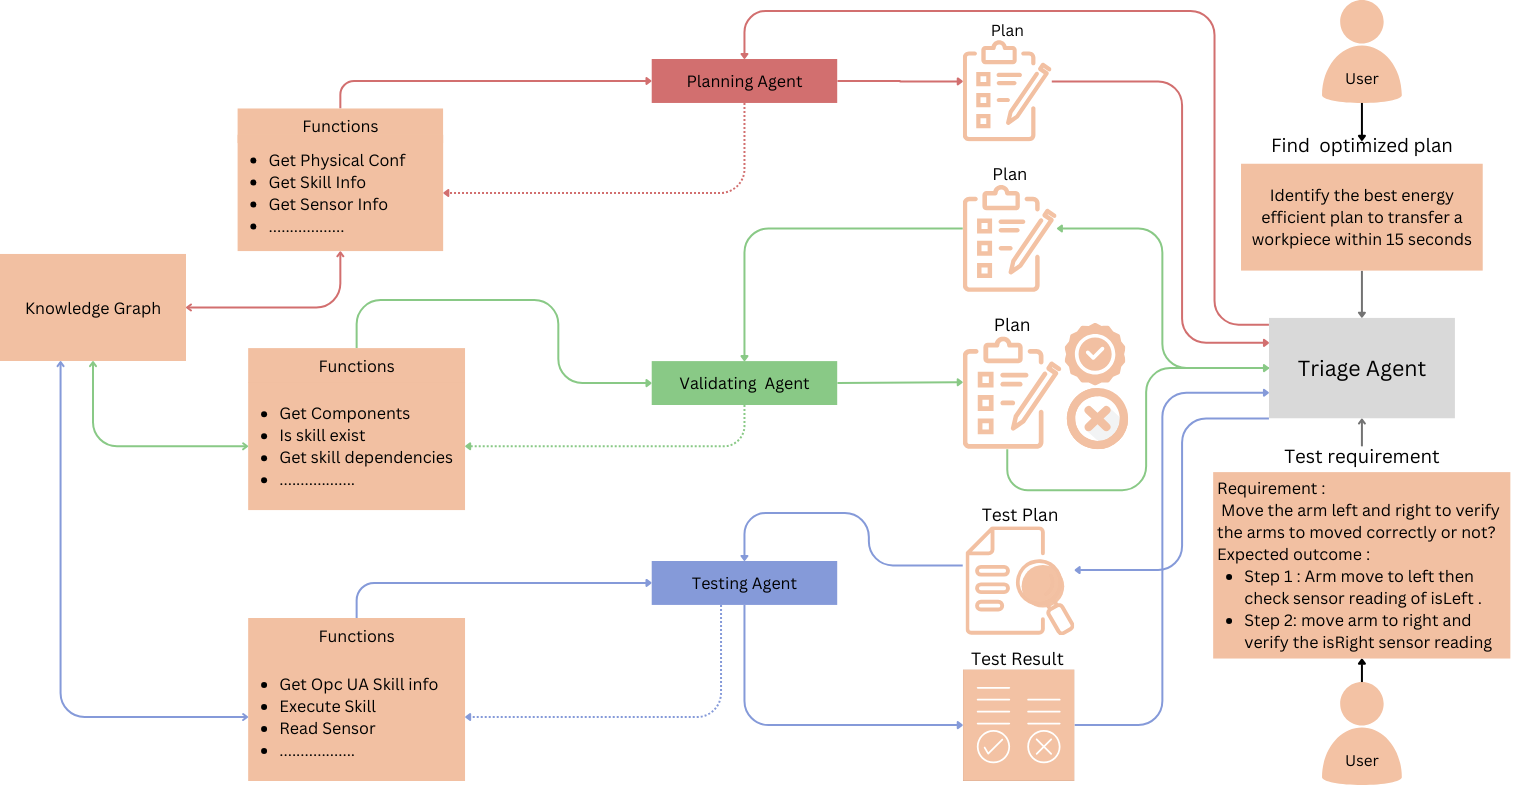
\includegraphics[width=1\textwidth]{MX_Papers/Paper13/images/arch.png}
        \caption{Multi-Agent system for plan, validate and test industrial control system}
        \label{fig:arch}
    \end{figure*}
    
    \section{Methodology}
    \label{methodlogy}
    
    This section presents the architecture and methodology of the proposed multi-agent system that enables intelligent planning, validation, and testing of industrial control systems (Fig. \ref{fig:arch}). The architecture uses a Knowledge Graph (KG) for semantic reasoning and integrates OPC UA communication to invoke services based on the IEC 61499 standard.
    
    \subsection{System Architecture Overview}
    
    The system architecture consists of a hierarchy of AI agents orchestrated by a \textit{Triage Agent}, which coordinates the \textit{Planning Agent}, \textit{Validating Agent}, and \textit{Testing Agent}. All agents share access to a centralized \textit{Knowledge Graph} that encodes the system’s configuration, available services (skills), execution costs, rules, and dependencies.
    
    The Triage Agent receives user requirements in natural language and delegates the responsibility of plan generation, validation, and testing to the respective agents. It also manages feedback and looping transitions between agents, ensuring iterative refinement until a valid and optimal plan is produced or a requirement-based test is completed.
    
    \subsection{Knowledge-Driven Planning}
    
    The \textit{Planning Agent} generates an optimized skill sequence to fulfill user-defined objectives. It queries the Knowledge Graph using semantic functions such as \textit{getPhysicalConfiguration()}, \textit{getSkillInfo()}, and \textit{getSensorInfo()} to collect relevant domain knowledge. To minimize noise in the Knowledge Graph, the Planning Agent leverages these targeted queries via function calling to extract only relevant and context-specific information, effectively filtering out irrelevant or conflicting data. It then reasons over the retrieved data, considering operational constraints such as energy usage, time, and dependency rules, and constructs a plan accordingly.
    
    
    \subsection{Plan Validation via Semantic Reasoning}
    
    The \textit{Validating Agent} is responsible for verifying whether the proposed plan adheres to the operational rules and resource constraints defined in the Knowledge Graph. It checks whether each skill is available, executable, and whether its dependencies are satisfied. The Validating Agent uses functions such as \textit{getSkillDependencies()},  \textit{ getExecutionRules()} and \textit{checkComponentAvailability()}. If the plan is invalid, the feedback is returned to the Triage Agent, which forwards it to the Planning Agent for replanning.
    
    \subsection{Automated Requirement-Based Testing}
    
    The \textit{Testing Agent} supports requirement-based system testing. The user provides a test requirement and the expected outcome. The system generates and validates a corresponding execution plan. Once validated, the Testing Agent executes the plan and verifies the observed system behavior against the expected outcome.
    
    \subsection{Operational Scenarios}
    
    \subsubsection{Optimized Planning Scenario}
    In this case, the user provides a requirement such as ``Generate an energy-efficient plan to transfer an object within 15 seconds." The Triage Agent activates the Planning Agent to retrieve configuration and skill metadata from the Knowledge Graph, reason over them, and construct an optimized sequence. The Validating Agent then checks for validity. If verified, the plan is returned to the user; otherwise, it is refined iteratively.
    
    \subsubsection{Requirement-Based Testing Scenario}
    Here, the user submits a testing requirement such as ``Move the robotic arm left and right and verify the motion via sensor feedback." The system generates a test plan and validates it. The Testing Agent then executes the skill sequence and verifies the outcome by reading real-time OPC UA variables (e.g., \texttt{rightSensor == True}). The outcome is compared to the expected result, and the final test verdict is reported to the user.
    
    
    \begin{figure*}
        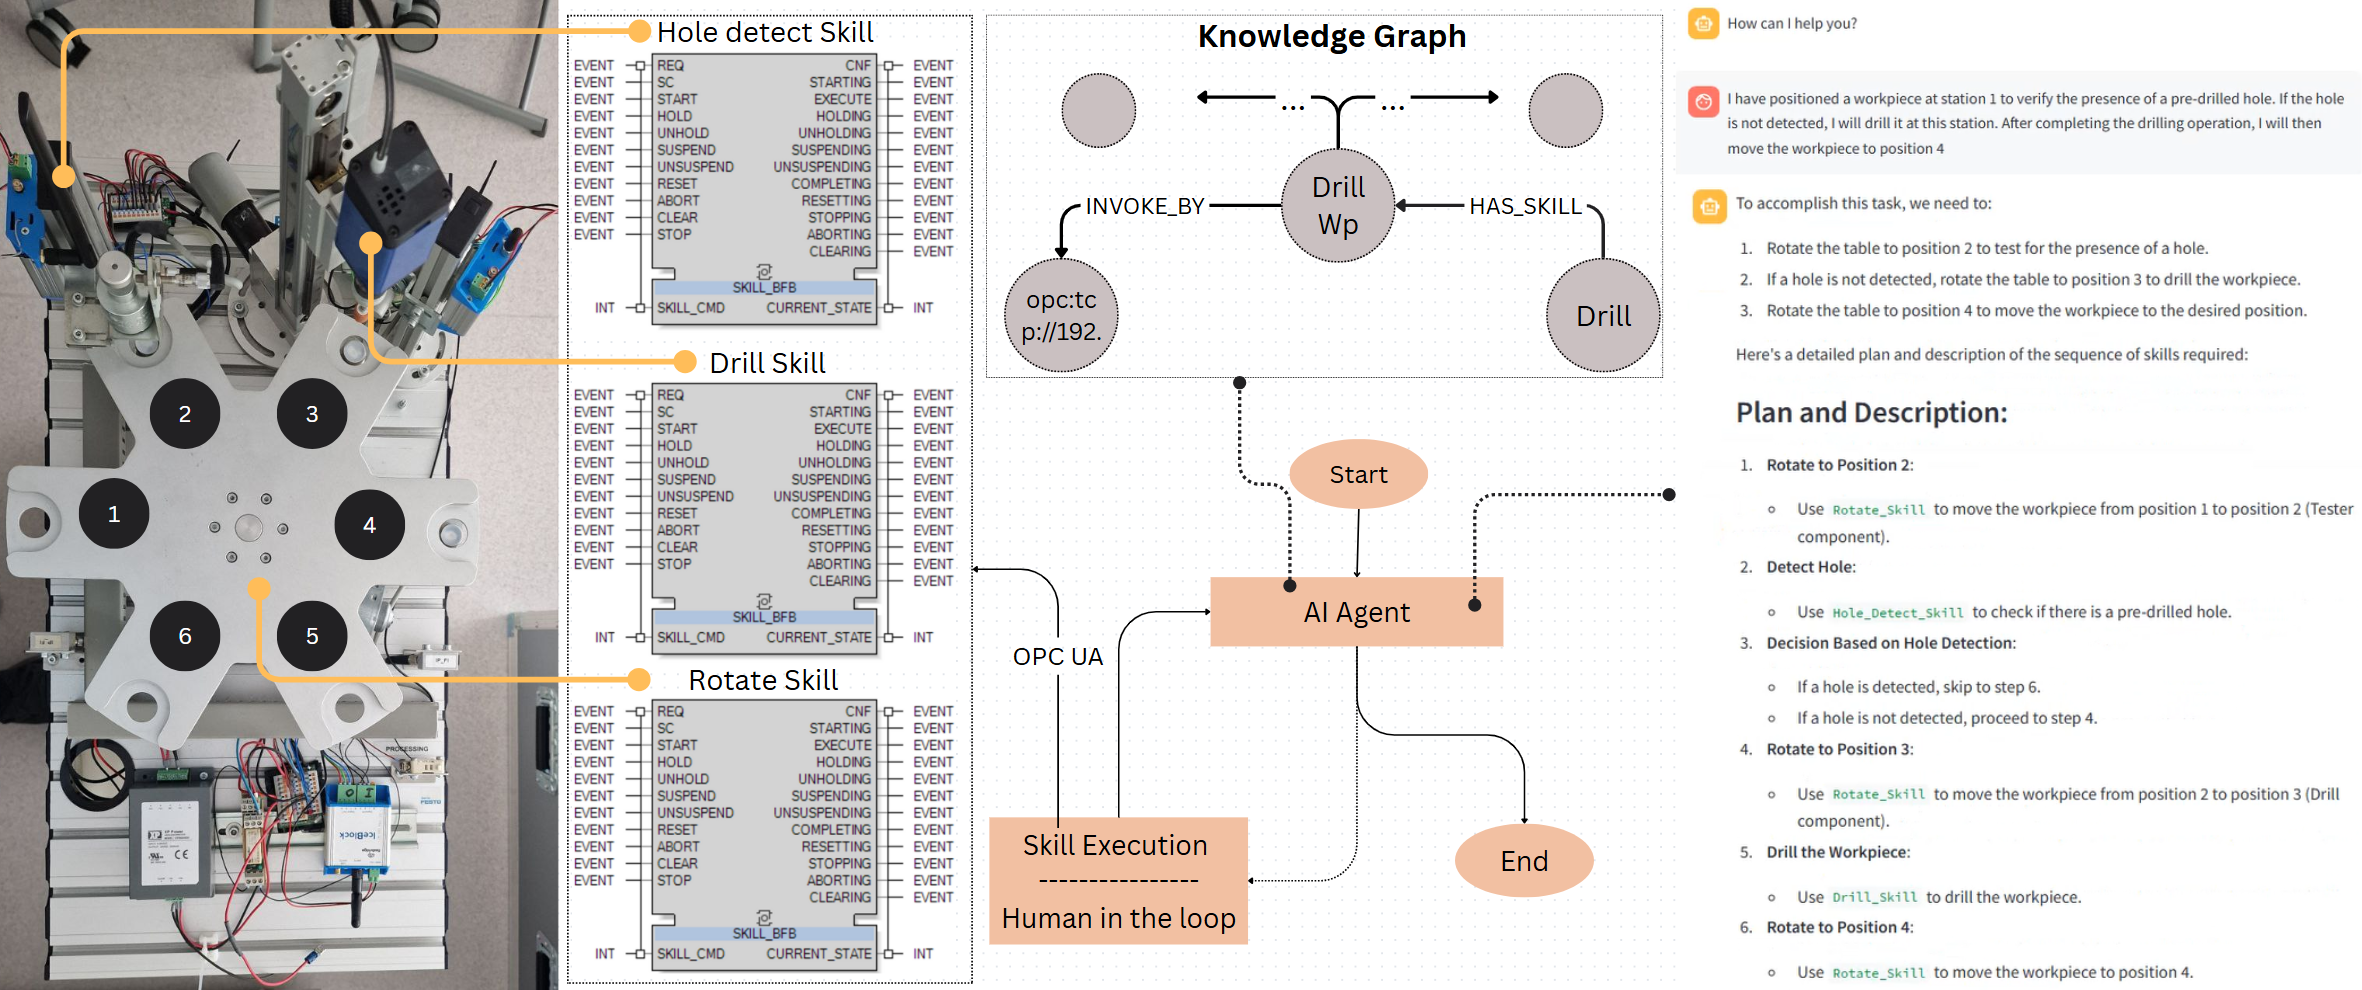
\includegraphics[width=1\textwidth]{MX_Papers/Paper13/images/PS_Arch.png}
        \caption{Intelligent Planning and Conditional Execution for Drilling in a Modular Processing Station}
        \label{fig:ps_arch}
    \end{figure*}
    
    
    
    
    \section{Case Study 1: Planning and Execution for Drilling in a Modular Processing Station}
    
    \subsection{System Overview}
    The Processing Station (Fig. \ref{fig:ps_arch}), located in the $AIC^3$ laboratory of Lulea University of Technology \cite{aiccubelab}, features a rotating table with six fixed positions. Among these, Position 2 is assigned to the \textit{Tester} unit, responsible for detecting holes in workpieces, while Position 3 hosts the \textit{Drill} unit for executing drilling operations. The rotating table supports one-step clockwise movements, with a complete cycle consisting of six rotations.
    
    Workpieces are initially loaded at Position 1. The primary objective of this system is to ensure that each workpiece is drilled. However, to enhance efficiency and conserve resources, the system first verifies whether the workpiece already has a hole and skips drilling if unnecessary. This  station is automated using IEC 61499 FBs, and all communication and control are facilitated using the OPC UA protocol.
    
    
    \subsection{Skill-Based Control in IEC 61499 for Modular Automation}
    
    In the skills-based engineering, \textit{a skill} represents a modular, reusable function that a control system can perform. These skills encapsulate well-defined operations—such as picking, placing, drilling, or welding—and are tied to specific hardware resources, such as robots, actuators, or sensors. 
    
    In this work, each skill is implemented using an \textit{IEC 61499 Function Block (FB)} (Fig. \ref{fig:ps_arch}). The internal execution logic of the Skill FB is managed through an \textit{Execution Control Chart (ECC)} that follows the \textit{ISA-88 procedural control model}. This standardization enables predictable behavior and seamless integration with other industrial automation systems. The Skill FB provides a standardized interface with input/output events and data, making it compatible with both \textit{human-machine interfaces (HMIs)} and external systems through \textit{OPC UA communication}.
    
    The Skill FB exposes control transitions such as \texttt{Start}, \texttt{Stop}, \texttt{Hold}, \texttt{Unhold}, \texttt{Suspend}, \texttt{Reset}, \texttt{Abort}, and \texttt{Clear}, and it maintains state consistency using signals like \texttt{EXECUTE}, \texttt{STARTING}, \texttt{STOPPING}, etc., as defined in the ECC state machine.
    
    
    To use a skill, the user can \textit{drag and drop the predefined Skill FB} into their IEC 61499 project. The Skill FB is then \textit{connected to existing control system function blocks} that implement the low-level operations (e.g., a custom FB for picking a workpiece). The Skill FB loads and manages the execution of these lower-level actions, allowing the control system to invoke complex sequences using a standard interface.
    
    
    \subsection{Objective and Skill Definitions}
    The intended task involves verifying the presence of a hole in a workpiece and performing a drilling operation only if the hole is absent. The system utilizes the following modular skills:
    \begin{itemize}
        \item \texttt{Rotate\_Skill}: Rotates the table one position clockwise.
        \item \texttt{Hole\_Detect\_Skill}: Engages the Tester to detect a hole in the workpiece.
        \item \texttt{Drill\_Skill}: Activates the Drill to create a hole.
    \end{itemize}
    
    The AI agent system is responsible for generating and executing an optimal and conditional sequence of these skills based on the workpiece's condition.
    
    \subsection{AI Agent-Based Planning and Validation}
    Upon receiving a high-level instruction such as ``Ensure the workpiece is drilled,'' the \textit{Triage Agent} initiates the planning process by delegating to the \textit{Planning Agent}. This agent accesses the shared Knowledge Graph using semantic queries (e.g., \texttt{getPhysicalConfiguration()}, \texttt{getSkillInfo()}) to retrieve the layout and functionality of the components.
    
    The Planning Agent generates the following initial plan:
    \begin{enumerate}
        \item Rotate the table to align Position 2 (Tester).
        \item Execute the \texttt{Hole\_Detect\_Skill}.
        \item If no hole is found:
        \begin{enumerate}
            \item Rotate the table to Position 3 (Drill).
            \item Execute the \texttt{Drill\_Skill}.
        \end{enumerate}
    \end{enumerate}
    
    The conditional nature of the plan introduces a feedback loop into the control sequence. The \textit{Validating Agent} reviews the plan to ensure its feasibility—checking component availability, validating preconditions for each skill, and confirming adherence to system constraints.
    
    \subsection{Testing and Dynamic Execution}
    After validation, the \textit{Testing Agent} sequentially executes each skill as specified in the plan. Prior to the execution of each skill, a \texttt{human-in-the-loop} mechanism is introduced, wherein the agent requests confirmation from a human operator before proceeding. Following the execution of each skill, the agent monitors feedback from the environment to dynamically determine the subsequent action based on the observed responses.For example, after executing the \texttt{Hole\_Detect\_Skill}, the agent reads the sensor result:
    \begin{itemize}
        \item If a hole is \textit{present}, the agent skips drilling.
        \item If a hole is \textit{absent}, the agent rotates to Position 3 and executes \texttt{Drill\_Skill}.
    \end{itemize}
    
    This dynamic decision-making process enables the system to operate adaptively, improving efficiency and reducing unnecessary operations.
    
    
    \begin{figure*}
        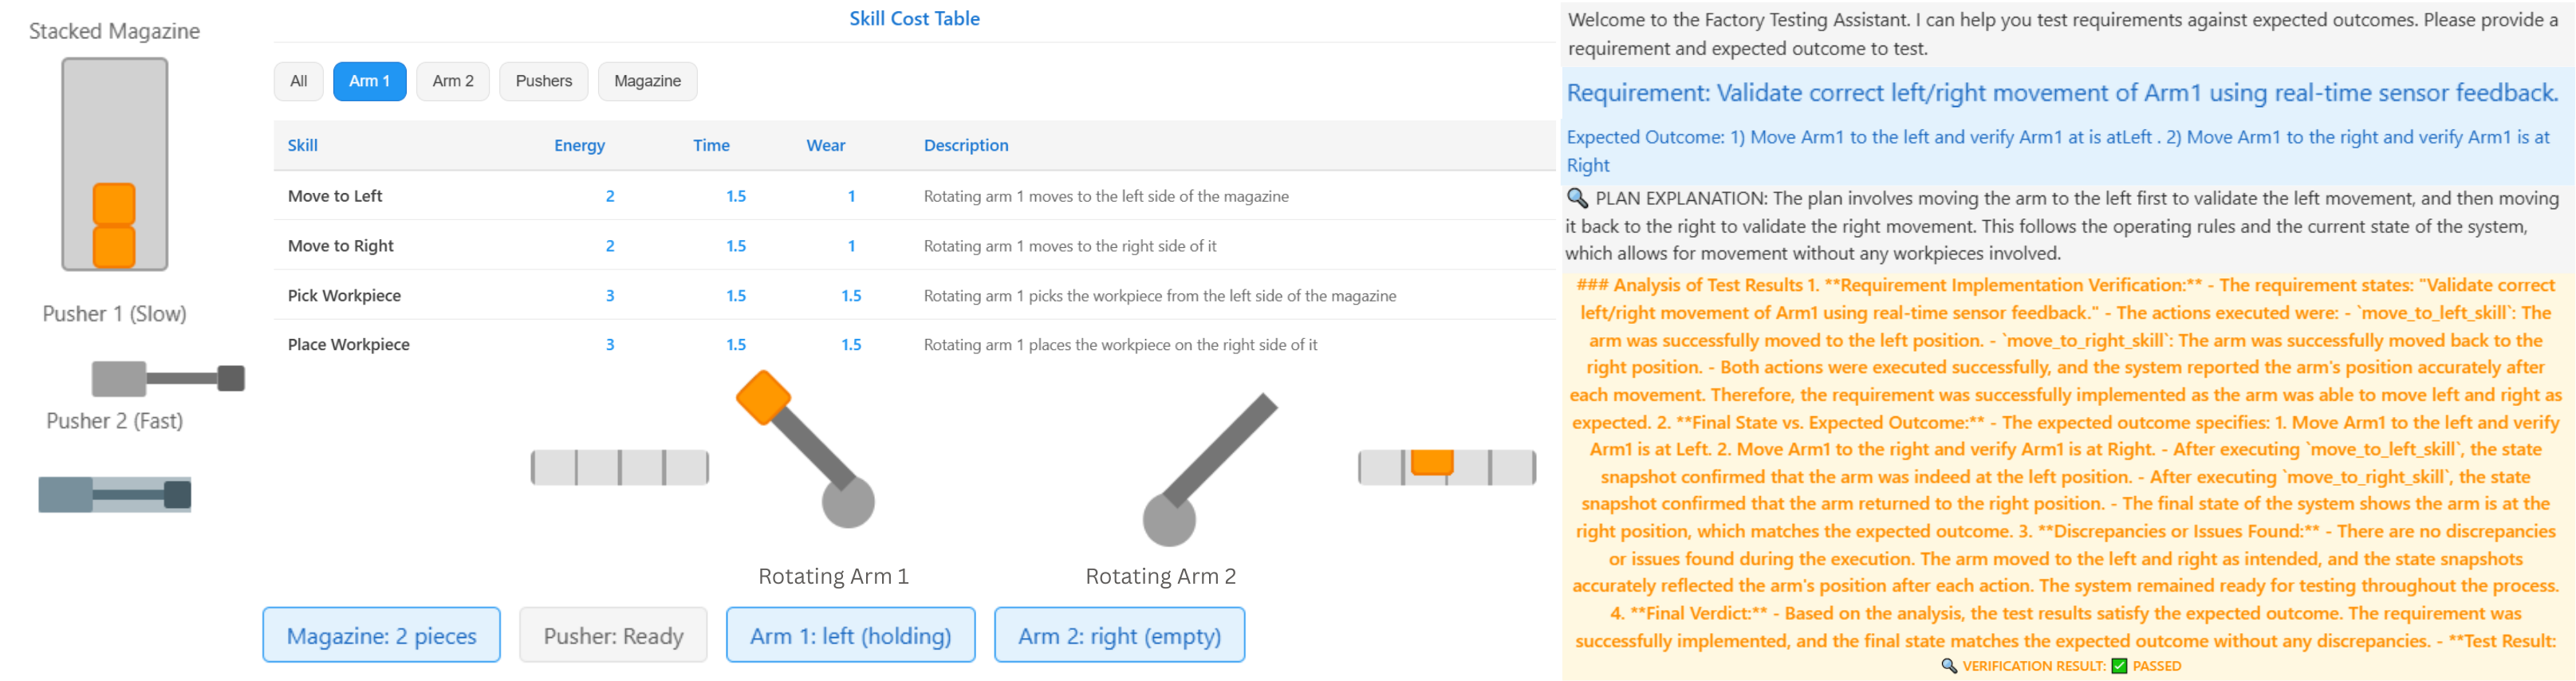
\includegraphics[width=1\textwidth]{MX_Papers/Paper13/images/DS_Arch.png}
        \caption{Requirement-Based Testing Distributing Station Automation Using AI Agents}
        \label{fig:ds_arch}
    \end{figure*}
    
    \section{Case Study 2: Distributing Station Automation Using AI Agents}
    
    This case study investigates the application of AI agent-based reasoning, planning, and testing to a modular distributing station. The station (Fig. \ref{fig:ds_arch}) comprises two rotating arms (Arm1 and Arm2), two pushers (Pusher1 and Pusher2), and a magazine unit capable of holding up to six workpieces. Each component exposes OPC UA method interfaces for control and sensor variables for state monitoring.
    
    \subsection{System Overview}
    Each skill is defined by its associated OPC UA method node, and it includes metadata such as energy, time, and wear cost. The AI architecture incorporates a Triage Agent, Planning Agent, Validating Agent, and Testing Agent, all sharing access to a centralized Knowledge Graph (KG). The KG encodes system structure, operational rules, skill costs, and sensor information.
    
    \subsection{Scenario 1: Energy-Efficient Transfer Plan Under Time Constraint}
    
    \texttt{Objective:} Generate the most energy-efficient plan to transfer a workpiece from the magazine to the right side of the system within \textit{15 seconds}.
    
    \texttt{Method:}
    \begin{itemize}
        \item The Triage Agent interprets the instruction and delegates planning.
        \item The Planning Agent queries the KG for skill metadata and current states.
        \item The Validating Agent checks for rule conformity, including movement constraints and energy budgets.
    \end{itemize}
    
    \begin{table}[h]
    \centering
    \caption{Energy-Efficient Transfer Plan (Within 15s)}
    \begin{tabular}{|c|l|c|c|c|c|}
    \hline
    \textbf{Step} & \textbf{Skill} & \textbf{Component} & \textbf{Time (s)} & \textbf{Energy} & \textbf{Wear} \\
    \hline
    1 & Load Magazine & Magazine & 2 & 2 & 0.5 \\
    2 & Push (slow) & Pusher1 & 3 & 1 & 0.5 \\
    3 & Move Left & Arm2 & 2 & 1 & 0.5 \\
    4 & Pick Workpiece & Arm2 & 2.5 & 2 & 1 \\
    5 & Move Right & Arm2 & 2 & 1 & 0.5 \\
    6 & Place Workpiece & Arm2 & 2.5 & 2 & 1 \\
    \hline
    \end{tabular}
    \label{tab:transfer_plan}
    \end{table}
    
    \texttt{Result:} The plan (TABLE \ref{tab:transfer_plan}) executes within 14 seconds and consumes 9 energy units, meeting both timing and energy requirements.
    
    \subsection{Scenario 2: Requirement-Based Testing of Arm Movement}
    
    \texttt{Objective:} Validate correct left/right movement of Arm1 using real-time sensor feedback.
    
    \texttt{Test Requirement:}
    \begin{enumerate}
        \item Move Arm1 to the left and verify \texttt{Arm1.isLeft == True}.
        \item Move Arm1 to the right and verify \texttt{Arm1.isRight == True}.
    \end{enumerate}
    
    \begin{table}[!t]
    \footnotesize
    \caption{Arm1 Motion Test Plan}
    \label{tab:test_plan}
    \begin{tabular}{|c|p{1.4cm}|p{2.8cm}|p{2.4cm}|}
    \hline
    \textbf{Step} & \textbf{Action} & \textbf{NodeId} & \textbf{Expected Sensor State} \\
    \hline
    1 & Move Left   & ns=2;s=Arm1.MoveLeft   & Arm1.isLeft = True \\
    2 & Verify      & ns=2;s=Arm1.IsLeft     & True \\
    3 & Move Right  & ns=2;s=Arm1.MoveRight  & Arm1.isRight = True \\
    4 & Verify      & ns=2;s=Arm1.IsRight    & True \\
    \hline
    \end{tabular}
    \end{table}
    
    \texttt{Result:} Sensor readings matched expectations, confirming actuator and sensor integrity. The test was successfully passed (TABLE \ref{tab:test_plan}).
    
    \section{ Evaluation of AI Agent }
    \label{sec: Evaluation}
    
    The evaluation of the AI agent, powered by the GPT-4o mini model, was carried out using 50 representative samples. The agent’s performance was assessed across three core dimensions, with all trajectories manually verified by human evaluators. \textit{Final response evaluation} focused on the agent’s ability to generate correct and efficient plans from natural language instructions, considering task success, energy efficiency, and time constraints. \textit{Single step evaluation} examined individual decisions such as tool selection and input generation to identify step-wise errors and enhance system traceability. \textit{Trajectory evaluation} analyzed the full sequence of actions for logical consistency and alignment with expected tool usage paths, as confirmed by human reviewers.
    
    
    \begin{table}[ht]
    \centering
    \caption{Evaluation Results of GPT-4o Mini-based AI Agent (50 Samples)}
    \begin{tabular}{|l|l|c|}
    \hline
    \textbf{Evaluation Type} & \textbf{Metric} & \textbf{Result} \\
    \hline
    \multirow{1}{*}{Final Response} 
        &  Plan Generation Accuracy & 94\%  \\
    \hline
    \multirow{2}{*}{Single Step} 
        & Function Selection Accuracy & 92\% \\
        & Input Argument Accuracy & 88\% \\
    \hline
    \multirow{1}{*}{Trajectory} 
        & Exact Skills Call Sequence Match & 86\% \\
    
    \hline
    \end{tabular}
    \label{tab:evaluation_results}
    \end{table}
    
    
    
    \section{Conclusion and future work}
    \label{sec:conclusion}
    
    This paper introduced a knowledge-driven AI agent framework for reasoning, planning, and testing industrial automation systems using natural language instructions. The multi-agent architecture—featuring dedicated planning, validation, and testing agents—proved more effective than single-agent setups by enabling modularity, feedback loops, and scalability. Generative AI outperformed traditional human approaches by reducing manual effort, interpreting intent in real time, and generating optimized, validated execution plans. Together, these advances highlight the potential of AI agents to enable intelligent, efficient, and scalable automation.
    
    
    In future work, we aim to extend this system by incorporating open-source LLM models to promote transparency and reproducibility. Benchmarking these models against proprietary alternatives will guide further development. Additionally, we plan to improve the reasoning capabilities of the agent through Reinforcement Learning with Human Feedback (RLHF). Data collection efforts for this fine-tuning process are currently underway.
    
    \section{Acknowledgements}
    The authorship team would like to acknowledge the vision, support and guidance of the IEEE Industrial Electronics Society in conducting the Generative AI Hackathon under the leadership of Daswin De Silva and Lakshitha Gunasekara.
    
\clearpage
\putbib
\end{bibunit} 